\documentclass[conference]{IEEEtran}
\usepackage{amsmath,amssymb,graphicx,booktabs,array,url}
\usepackage[hidelinks]{hyperref}
\usepackage{cite}
\newcommand{\AURA}{\textsc{Aura}}
\title{AURA: Evaluating Disagreement-Aware Selective Multimodal Learning for Axial Spondyloarthritis in a Synthetic Benchmark}
\author{\IEEEauthorblockN{Anonymous author(s)}\IEEEauthorblockA{Author details withheld for review}}
\begin{document}
\maketitle
\begin{abstract}
Axial spondyloarthritis (axSpA) assessment depends on heterogeneous clinical, laboratory and imaging evidence that may be missing, noisy or discordant. We investigate whether inter-modality disagreement improves selective prediction after accounting for model confidence, modality availability and measurement quality. AURA combines bootstrapped modality-specific logistic experts, validation-fitted inverse-error fusion, probability recalibration, an error-ranking model and exact modality-coalition attributions. We construct a synthetic benchmark with ten independent seeds, 10,000 development-population records per seed, seven observation or population conditions and eight model configurations. Across conditions, AURA attains mean area under the receiver operating characteristic curve (AUROC) of 0.8271, Brier score of 0.1614 and area under the risk-coverage curve (AURC) of 0.1217. Its learned error ranker reduces AURC relative to entropy-only ranking (paired difference $-0.00424$, 95\% seed-level interval $[-0.00568,-0.00280]$). Adding disagreement to the matched error ranker yields a much smaller difference ($-0.00014$, interval $[-0.00069,0.00041]$); early-fusion logistic regression achieves lower overall AURC (0.1193). Under combined degradation, AURA AUROC falls to 0.7422. The findings support evaluation of transparent selective fusion while providing no clear evidence for incremental disagreement utility in this simulator. The benchmark uses no patient records; its results do not establish clinical diagnostic accuracy or readiness.\end{abstract}
\begin{IEEEkeywords}
axial spondyloarthritis, selective prediction, multimodal fusion, missing modalities, uncertainty, explainable AI, simulation
\end{IEEEkeywords}
\section{Introduction}
Axial spondyloarthritis is an inflammatory rheumatic condition affecting the axial skeleton. Its assessment incorporates patient history, laboratory findings and imaging of the sacroiliac joints. Clinical guidance emphasizes that negative HLA-B27 and normal inflammatory markers cannot independently exclude disease \cite{nice}. Furthermore, imaging findings can overlap with non-inflammatory conditions and classification criteria should not be treated as a diagnostic reference standard \cite{mri,asas}. These properties motivate decision-support research that explicitly represents incomplete and potentially inconsistent evidence.

Machine learning (ML) has been studied in axSpA for both imaging interpretation and clinical prediction \cite{adams,meta}. Recent diagnostic systems combine imaging and risk features, including multicenter deep learning \cite{xie}, conventional random forests \cite{rf}, TabNet \cite{tabnet} and explainable segmentation-assisted decision support \cite{cdss}. Accordingly, neither multimodal integration nor interpretability alone constitutes a novel technical claim. More generally, quality-aware fusion and cross-view conflict modelling are established directions in multimodal learning \cite{tmc,qamoe,aemrl}.

A related problem concerns \emph{selective prediction}: a model may defer a decision rather than output an uncertain classification. The important question is whether a proposed uncertainty statistic identifies errors more effectively than confidence alone, especially in the presence of incomplete data. Agreement between individually unreliable sources does not guarantee correctness; conversely, disagreement may represent useful complementary evidence rather than error. This motivates a matched comparison that holds predicted probabilities constant while varying the error-ranking features.

This work proposes AURA (a reliability and uncertainty-aware assessment framework) as a lightweight, auditable test bed for this question. Its contributions are: (i) a reproducible axSpA-inspired synthetic benchmark with distinct missingness, noise and population-shift conditions; (ii) a validation-fitted risk-weighted fusion and selective ranking pipeline; (iii) an explicit disagreement ablation with paired seed-level analysis and strong early-fusion controls; and (iv) two complementary, algebraically checked explanation views. The goal is methodological, not a clinical diagnostic claim. The study evaluates a binary simulated class rather than assigning specific differential diagnoses.
\section{Related Work and Research Gap}
\subsection{AxSpA clinical and imaging models}
A clinical diagnostic review describes the limitations of isolated laboratory and imaging findings \cite{clinical}. A meta-analysis examines AI tools across radiography, CT and MRI \cite{meta}. Xie et al. combine 3D MRI representations with clinical predictors in a four-center cohort of 1,294 patients \cite{xie}. A rheumatological routine-care study uses random forests and imputation on 939 records \cite{rf}. TabNet combines structured SIJ findings with clinical variables in 942 patients \cite{tabnet}; MRI and clinical models have also been investigated in HLA-B27-negative disease \cite{negative}. A more recent clinical decision support architecture combines multi-sequence MRI with risk scores and segmentation-based interpretation \cite{cdss}. These studies motivate the feature groups, but their reported clinical discrimination cannot be compared directly with results from generated records.
\subsection{Missingness, reliability and selective prediction}
Multimodal learning taxonomies distinguish representation, fusion and alignment \cite{bal}. Modality dropout and heterogeneous modality aggregation offer approaches to unavailable inputs \cite{moddrop,hemis}. Clinical multimodal robustness remains an active area, including attention-based fusion \cite{attention} and a recent mechanism-level review \cite{missingreview}. Trusted multi-view classification uses dynamic evidential fusion \cite{tmc}; multimodal dynamics estimates sample-specific informativeness \cite{dynamics}. QA-MoE integrates quality scoring, stable subset selection and expert routing, including abstaining experts \cite{qamoe}. Conflict-aware calibration has likewise been investigated \cite{aemrl}. These methods are important conceptual competitors, but this paper does not claim to reproduce or outperform their original implementations.

Reject-option classification and risk-coverage evaluation are established \cite{selective}. Calibration \cite{guo}, ensemble-based uncertainty \cite{ensembles} and robustness under dataset shift \cite{ovadia} inform the evaluation. Recent multimodal clinical selective prediction work highlights failure modes caused by calibration and class imbalance \cite{lopez}. We therefore distinguish class-probability calibration from error-ranking performance and report both coverage-matched and fixed-threshold outcomes.
\begin{table}[t]
\caption{Closest conceptual comparators (not matched-data results).}
\label{tab:related}
\centering\footnotesize
\begin{tabular}{@{}p{0.19\columnwidth}p{0.34\columnwidth}p{0.36\columnwidth}@{}}\toprule
Work & Established contribution & Distinction in this study\\\midrule
Xie et al. \cite{xie} & MRI + clinical predictors & Synthetic evidence stress tests\\
TabNet \cite{tabnet} & Structured MRI + risk & Matched selective ranking\\
CDSS \cite{cdss} & MRI + explainable segmentation & Coalition explanations, no raw MRI\\
TMC \cite{tmc} & Dynamic evidential fusion & Lightweight inverse-error gate\\
QA-MoE \cite{qamoe} & Quality-aware expert selection & Explicit disagreement-only ablation\\
AEMRL \cite{aemrl} & Conflict-aware calibration & Test whether disagreement adds value\\
Lopez et al. \cite{lopez} & Clinical selective prediction & Binary synthetic axSpA-inspired task\\\bottomrule
\end{tabular}
\end{table}
\subsection{Scope of the gap}
Table~\ref{tab:related} summarizes the nearest methodological and clinical precedents identified in a targeted scoping search. The associated research matrix records 44 publications/resources across clinical diagnosis, axSpA AI, data access, fusion, uncertainty, explanation and reporting. Searches used combinations of axSpA/ankylosing spondylitis, diagnosis, MRI, missing modality, clinical prediction, conflict, calibration and selective classification, with foundational papers retained irrespective of publication year. The matrix is based on metadata, abstracts and selected accessible full-text material; it is not an exhaustive systematic review. We do not claim that no prior study has tested disagreement. Our specific question is whether weighted prediction dispersion adds incremental error-ranking value on an explicit axSpA-inspired stress benchmark after controlling for confidence, availability and quality.
\section{Problem Formulation}
Let $Y\in\{0,1\}$ be a latent simulated class and $X=(X_C,X_L,X_I)$ represent clinical, laboratory and structured imaging evidence. Let $m_k\in\{0,1\}$ indicate modality availability and $q_k\in[0,1]$ denote an observed quality proxy for $k\in\{C,L,I\}$. The objective is to estimate a class probability $\hat p$ and an error-ranking score $u$ for records with at least one available modality. The selective classifier is
\begin{equation}
 h_\tau(X,m,q)=\begin{cases}\bot,&\sum_km_k=0\ \text{or}\ u>\tau,\\\mathbb{1}[\hat p\geq 0.5],&\text{otherwise}.\end{cases}
\end{equation}
Here $\bot$ represents deferral, not a negative class. The implementation evaluates nonempty masks only; an operational system would have to handle zero evidence explicitly. The threshold 0.5 is a computational convention, not a clinical referral cutoff.

For error indicator $e_i=\mathbb{1}[\hat y_i\neq y_i]$, coverage $c(\tau)$ and selective risk $r(\tau)$ are
\begin{align}
c(\tau)&=n^{-1}\sum_i\mathbb{1}[u_i\leq\tau],\\
r(\tau)&=\frac{\sum_i e_i\mathbb{1}[u_i\leq\tau]}{\sum_i\mathbb{1}[u_i\leq\tau]},
\end{align}
where risk is undefined at zero coverage. AURC is calculated empirically by sorting records from lowest to highest error score and averaging cumulative error over all retained-set sizes. Lower AURC means better selective performance, conditional on the underlying classifier.

Three questions guide evaluation: RQ1: Does learned fusion improve discrimination/calibration relative to equal and observed-quality weighting? RQ2: Does learned error ranking improve AURC relative to entropy? RQ3 (primary comparison): Does disagreement improve AURC relative to an otherwise identical ranker? The analysis is exploratory, not prospectively preregistered.
\section{Proposed AURA Method}
\subsection{Modality experts and reliability gate}
For each modality, five logistic regression models are fit on independent bootstrap resamples of the expert-training partition, using standardized features and quality. Their mean and variance are
\begin{align}
p_k &= B^{-1}\sum_{b=1}^{B}p_{kb},\quad B=5,\\
v_k &= B^{-1}\sum_{b=1}^{B}(p_{kb}-p_k)^2.
\end{align}
Variance is a heuristic measure of model instability, not a full Bayesian decomposition. Using a disjoint gate partition, ridge regression estimates the squared probability error $\ell_k=(p_k-Y)^2$ from $z_k=[q_k,|p_k-0.5|,q_k|p_k-0.5|,q_k^2]$. For the fitted estimate $g_k(z_k)$, define
\begin{align}
a_k&=\{\max(0.03,g_k(z_k))\}^{-1},\\
w_k&=\frac{m_ka_k}{\sum_j m_ja_j},\qquad p_f=\sum_kw_kp_k.
\end{align}
The gate uses ridge regularization $\alpha=5$. The inverse predicted error is a transparent heuristic: for independent, unbiased estimators with known error variances, inverse-variance weighting minimizes the variance of a weighted mean. Here errors may be biased and correlated, so that optimality argument does not apply; the gate is evaluated empirically. Clipping prevents arbitrarily large weights. Missing inputs receive zero weight. Equal and quality-weighted fusion use the identical experts but replace $a_k$ with 1 and $q_k$, respectively.
\subsection{Calibration and disagreement}
A separate calibration partition fits a logistic recalibrator
\begin{equation}
\hat p=\sigma(b_0+b_1\operatorname{logit}(\operatorname{clip}(p_f))),
\end{equation}
where probability clipping uses $10^{-6}$ and $1-10^{-6}$. All comparator probability outputs receive the same type of recalibration. This avoids conflating the choice of fusion with the presence of calibration.

Disagreement is the weighted dispersion of expert means,
\begin{equation}
D=\sum_kw_k(p_k-p_f)^2=\sum_kw_kp_k^2-p_f^2.
\end{equation}
Since each $p_k\in[0,1]$, $0\leq D\leq1/4$; thus $4D\in[0,1]$. A single available modality has $D=0$, which does not imply high reliability. Two models that make similarly erroneous predictions also produce low disagreement. These cases motivate the inclusion of other uncertainty features.
\subsection{Matched error ranking}
On the dedicated uncertainty-development partition, fit standardized logistic regressions to predict $e=\mathbb{1}[\mathbb{1}[\hat p\geq0.5]\neq Y]$. The baseline feature vector is
\begin{equation}
 t_0=[H_2(\hat p),\sum_kw_kv_k,\tfrac{1}{3}\sum_km_k,\bar q,m_C,m_L,m_I],
\end{equation}
where $H_2$ is binary entropy in bits and $\bar q=\sum_k m_k q_k/\sum_km_k$. The full ranker adds $4D$ to $t_0$. Both rankers use the same model class, default regularization and data. The entropy-only comparator ranks solely by $H_2$. All three share exactly the same $\hat p$ and class predictions, enabling isolation of ranking effects from classification effects. The fixed operating threshold is the 80th percentile of full-ranker scores on the ranker-development partition; this is an in-sample threshold selection and is not a risk guarantee.
\subsection{Two-level explanation}
For the set $A$ of available modalities, define the coalition value $V(S)$ for $S\subseteq A$ by renormalizing existing weights over $S$ and recalibrating the resulting score. Set $V(\emptyset)$ to the recalibrated score at raw probability 0.5. The exact Shapley contribution \cite{shap} of modality $k$ is
\begin{equation}
\phi_k=\sum_{S\subseteq A\setminus\{k\}}\frac{|S|!(|A|-|S|-1)!}{|A|!}[V(S\cup\{k\})-V(S)].
\end{equation}
With at most three modalities, exact enumeration is feasible. The attributions sum to $V(A)-V(\emptyset)$, but depend on the chosen reference and masking rule. They are model-specific, not causal. For within-modality interpretation, standardized feature contributions $\beta_j z_j$ of the first logistic expert member are reported on its logit scale. This view is exact for that member, not a decomposition of the entire ensemble. The two explanation levels are deliberately not added together.
\begin{figure}[t]
\centering
\setlength{\fboxsep}{3pt}
\begin{tabular}{c}
\fbox{\parbox{.91\columnwidth}{\centering Clinical $\mid$ Laboratory $\mid$ Structured imaging}}\\[-1pt]
$\downarrow$\\
\fbox{\parbox{.91\columnwidth}{\centering Bootstrap experts: $p_k,v_k$; observed $m_k,q_k$}}\\[-1pt]
$\downarrow$\\
\fbox{\parbox{.91\columnwidth}{\centering Ridge error gate $\rightarrow$ masked fusion $\rightarrow$ calibration}}\\[-1pt]
$\downarrow$\\
\fbox{\parbox{.91\columnwidth}{\centering Entropy, variance, quality, mask, disagreement}}\\[-1pt]
$\downarrow$\\
\fbox{\parbox{.91\columnwidth}{\centering Error ranker $\rightarrow$ classify or defer\\ Coalition and expert-logit explanations}}\\
\end{tabular}
\caption{AURA computational architecture. The output is a simulated binary assessment, not a clinical diagnosis.}
\label{fig:arch}
\end{figure}
\section{Synthetic Benchmark and Experimental Protocol}
\subsection{Data provenance and generation}
The DESIR cohort is a potential source of longitudinal diagnostic evidence, but access is subject to request and governance \cite{desir}. No suitable matched open clinical/laboratory/imaging dataset was obtained in the present study. Therefore, all observations are generated by code. The generator is inspired by qualitative clinical evidence, not fitted to patient-level distributions or published diagnostic likelihood ratios. No medical record, raw image, identifiable data or physician diagnosis was used.

For each seed, sample 10,000 latent labels $Y\sim\operatorname{Bernoulli}(0.40)$ and an inflammation proxy $Z\sim\mathcal N(0.8Y,1)$. A latent mimic indicator $J$ is sampled with probability 0.17 for negative cases and 0.08 for positives, creating shared non-specific evidence. Let $G\sim\mathcal N(0,1)$ be a second latent factor. Binary observations follow $X_j\sim\operatorname{Bernoulli}(\sigma(a_j+b_jY+c_jZ+d_jJ+e_jG))$; continuous proxies are affine combinations of the latent variables with unit Gaussian noise. Table~\ref{tab:coeff} specifies the clean generator. The label is sampled before features; it is not the output of a clinical classification rule or of AURA. Nevertheless, the chosen causal structure can favor certain learners and is not claimed to reproduce disease mechanisms.
\begin{table}[t]
\caption{Synthetic feature generator coefficients. B = Bernoulli with logistic link; N = Gaussian with unit variance.}
\label{tab:coeff}
\centering\footnotesize
\begin{tabular}{@{}llrrrrr@{}}\toprule
Feature & Type & $a$ & $b$ & $c$ & $d$ & $e$\\\midrule
Stiffness & B & -.9 & 1.1 & .55 & .8 & 0\\
Movement relief & B & -.9 & 1.5 & .3 & .3 & 0\\
Night pain & B & -1 & 1.1 & .5 & .7 & 0\\
Extra-articular & B & -2 & 1.35 & 0 & 0 & .2\\
HLA-B27 & B & -2.2 & 2.15 & 0 & 0 & .3\\
CRP proxy & N & 0 & .55 & .48 & .22 & 0\\
ESR proxy & N & 0 & .35 & .52 & .22 & 0\\
BME & B & -1.8 & 1.65 & .65 & 1.9 & 0\\
Erosion & B & -2.2 & 1.8 & .42 & .35 & 0\\
Structural proxy & N & 0 & .55 & .35 & .45 & 0\\\bottomrule
\end{tabular}
\end{table}

Quality $q_k$ is independently sampled from $\mathrm{Beta}(5,2)$ under the reference acquisition mechanism. For each binary feature, its clean value is flipped with probability $0.36(1-q_k)$; continuous features receive independent zero-mean Gaussian perturbations with standard deviation $1.2(1-q_k)$. CRP, ESR and structural features are dimensionless proxies, not clinically interpretable laboratory or radiology measurements. The latent mimic flag is excluded from model inputs. Quality is an observed simulator variable; in clinical practice an independently validated quality estimator would be required.
\subsection{Stress conditions}
\begin{table}[t]
\caption{Seven evaluation conditions; masks with zero modalities are repaired by uniformly selecting one modality.}
\label{tab:scen}
\centering\footnotesize
\begin{tabular}{@{}p{.26\columnwidth}p{.67\columnwidth}@{}}\toprule
Condition & Observation/population intervention\\\midrule
Complete & All three modalities, reference quality\\
MCAR30 & Independent pre-repair dropout 30\%\\
MCAR50 & Independent pre-repair dropout 50\%\\
Quality & Quality changes to $\mathrm{Beta}(2,4)$\\
Selective & Lab/MRI acquisition depends on symptoms and latent class\\
Mimic & Prevalence 25\%, negative mimic rate 48\%\\
Combined & Mimic population, low quality, 40\% dropout\\\bottomrule
\end{tabular}
\end{table}
Table~\ref{tab:scen} summarizes stress conditions. For selective acquisition, clinical evidence is always present and the laboratory and imaging acquisition probabilities are $\sigma(-0.7+1.15X_1+0.55Y)$ and $\sigma(-1.1+1.4X_2+0.7Y)$, respectively, using clean clinical indicators. Dependence on unobserved $Y$ intentionally creates missing-not-at-random (MNAR) stress. In the mimic and combined conditions, new independent populations are sampled with positive prevalence 0.25 and negative mimic probability 0.48; all other generator coefficients remain fixed. This is not a validated model of specific infectious, mechanical or degenerative diagnoses. Conditions sharing the reference population reuse the same held-out records but sample independent observation perturbations. For every condition, at least one modality is retained; nominal dropout rates therefore differ from realized missingness.
\subsection{Data splitting, comparators and metrics}
Ten seeds (20261124 through 20261133) are run independently. Each reference population is partitioned into 5,000 expert-training, 1,500 gate, 1,000 calibration, 1,000 ranker-development and 1,500 held-out records. Training, gate, calibration and ranker observations use reference quality and nominal 22\% dropout (experts are trained using available generated measurements before masking). The shifted evaluation populations contain 1,500 new observations per seed and condition. Model fitting never uses test labels. The experiment uses the same partitions and observed test features for every configuration within each seed and condition.

Eight configurations are evaluated: mask-aware early logistic regression, random forest (80 trees, minimum leaf size 8), histogram gradient boosting (100 iterations, at most 15 leaves), equal late fusion, quality late fusion, and three AURA rankers. Early fusion concatenates zero-filled features, mask indicators and masked quality. All models are calibrated using the dedicated calibration partition. Non-AURA comparators use entropy-based ranking. No hyperparameter optimization is performed. The small model set provides transparent controls, not an exhaustive state-of-the-art competition.

We calculate AUROC, average precision, Brier score, log loss, accuracy, ten-bin equal-width expected calibration error (ECE), AURC, selective risk at 80\% and 50\% coverage, and error detection AUROC. Fixed-coverage metrics use test-score ordering without labels to determine retained sets, while fixed-threshold metrics use the development-selected threshold. We report equal-weight macro means over conditions and seeds rather than pooling correlated records. For each paired AURC contrast, condition-level differences are first averaged within seed, then summarized with a two-sided 95\% Student-$t$ interval across ten seed means. These intervals measure variation under the stipulated generator, not clinical population uncertainty. Secondary comparisons are exploratory and unadjusted for multiplicity.
\section{Results}
\begin{table}[t]
\caption{Macro means across ten seeds and seven conditions. Best value in each column bolded; AUROC and error AUROC higher is better; other columns lower is better.}
\label{tab:macro}
\centering\footnotesize
\begin{tabular}{@{}lrrrrr@{}}\toprule
Model & AUROC & Brier & AURC & Risk80 & Err. AUC\\\midrule
Early logistic & \textbf{.8296} & \textbf{.1594} & \textbf{.1193} & .1812 & \textbf{.7214}\\
Early RF & .8185 & .1655 & .1306 & .1954 & .7144\\
Early HGB & .8184 & .1645 & .1295 & .1927 & .7130\\
Equal fusion & .8246 & .1629 & .1281 & .1829 & .7145\\
Quality fusion & .8249 & .1628 & .1280 & .1826 & .7141\\
AURA entropy & .8271 & .1614 & .1260 & \textbf{.1811} & .7170\\
AURA no $D$ & .8271 & .1614 & .1219 & .1835 & .7188\\
AURA full & .8271 & .1614 & .1217 & .1842 & .7184\\\bottomrule
\end{tabular}
\end{table}
\subsection{Fusion and selective prediction}
Table~\ref{tab:macro} reports all 560 seed-condition-configuration evaluations in aggregate. Relative to equal weighting, learned reliability fusion increases macro AUROC from 0.8246 to 0.8271 and decreases Brier score from 0.1629 to 0.1614. These differences are modest. Early logistic regression obtains the best macro discrimination, Brier score and AURC. AURA therefore does not dominate simpler baselines. The generator's approximately linear latent structure plausibly favors logistic models, but the cause of the performance difference is not established by this experiment.

The full ranker reduces macro AURC from 0.1260 (entropy only) to 0.1217. The paired seed-level difference is $-0.00424$ (95\% interval $[-0.00568,-0.00280]$). AURA full versus equal fusion yields $-0.00634$ ($[-0.00815,-0.00452]$), and versus early HGB yields $-0.00772$ ($[-0.01075,-0.00470]$). Unlike the comparison to entropy, these latter contrasts mix changes in classification and ranking. At 80\% coverage, AURA full risk (0.1842) is slightly higher than entropy-only AURA (0.1811). A lower integrated risk does not guarantee improvement at every coverage level.
\begin{figure}[t]
\centering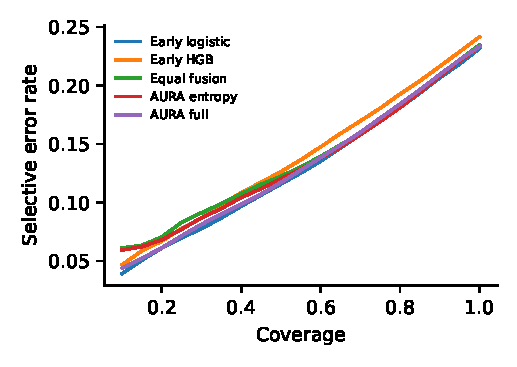
\includegraphics[width=\columnwidth]{figures/risk_coverage.pdf}
\caption{Mean selective risk versus coverage across conditions and seeds. Curves are sampled at coverage 0.10 to 1.00; AURC uses all ranks.}
\label{fig:rc}
\end{figure}
\subsection{Incremental disagreement contribution}
The primary matched ablation yields a mean AURC difference of $-0.00014$ (95\% interval $[-0.00069,0.00041]$) when adding disagreement to the error ranker. The interval includes zero; the experiment does not establish a reliable benefit. Error detection AUROC is 0.7184 with disagreement and 0.7188 without it. Both configurations share class probabilities and errors, so the observed difference is attributable to ranking rather than discrimination. In the combined shift condition the paired AURC difference is $-0.00080$ (interval $[-0.00285,0.00124]$); in the complete condition it is $+0.00007$ ($[-0.00012,0.00027]$). None provides convincing evidence that dispersion adds predictive value after other features. The results do not imply that disagreement is useless in every setting; they constrain the claim to this implementation and simulator.
\begin{table}[t]
\caption{AURA full by scenario. Cov. and risk use the fixed development-selected score threshold; all entries are seed means.}
\label{tab:stress}
\centering\footnotesize
\begin{tabular}{@{}lrrrrr@{}}\toprule
Condition & AUROC & ECE & AURC & Cov. & Risk\\\midrule
Complete & .8828 & .0472 & .0818 & .8836 & .1608\\
MCAR30 & .8457 & .0309 & .1092 & .7697 & .1643\\
MCAR50 & .8159 & .0489 & .1340 & .7166 & .1791\\
Quality & .8198 & .0304 & .1331 & .7001 & .1795\\
Selective & .8288 & .0385 & .1266 & .7661 & .1816\\
Mimic & .8543 & .1139 & .0859 & .8744 & .1642\\
Combined & .7422 & .1439 & .1816 & .5956 & .2031\\\bottomrule
\end{tabular}
\end{table}
\begin{figure}[t]
\centering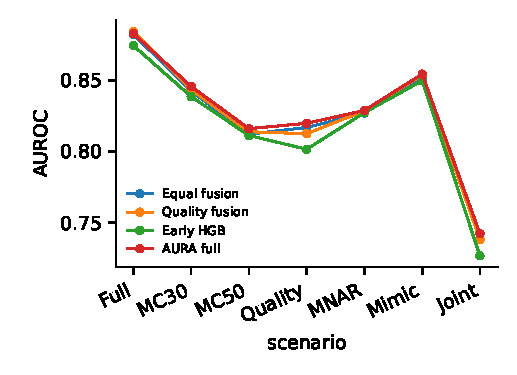
\includegraphics[width=\columnwidth]{figures/robustness.pdf}
\caption{Discrimination under missingness and shift; values averaged across seeds.}
\label{fig:robust}
\end{figure}
\subsection{Stress response and threshold transport}
Table~\ref{tab:stress} and Fig.~\ref{fig:robust} show declining discrimination under increased missingness and reduced quality. In the complete condition, mean AUROC is 0.8828 and AURC is 0.0818. In the combined shift, these deteriorate to 0.7422 and 0.1816 respectively, with ECE increasing from 0.0472 to 0.1439. In the mimic-shift condition, mean ECE is 0.1139 despite AUROC 0.8543. A reasonably strong ranking metric can coexist with substantial calibration error.

The fixed threshold retains 88.36\% of complete-condition records and 59.56\% in the combined shift. The corresponding retained risks are 16.08\% and 20.31\%. The threshold does not deliver invariant coverage or error control. The nominal 50\% pre-repair dropout yields a mean of 1.629 observed modalities, versus 2.130 under 30\% dropout. The low-quality combined condition has mean observed quality 0.334, compared with 0.715 for complete data. These audits verify the intended stress directions, not clinical plausibility.
\subsection{Explanation and implementation checks}
For 100 complete-condition records from the first seed, exact coalition attributions reconstruct the calibrated score relative to the empty-coalition reference within numerical tolerance ($10^{-9}$). As an example, one simulated record has reference 0.5959 and predicted score 0.3964; contributions from clinical, laboratory and imaging groups are $+0.2433,-0.1992,-0.2435$, respectively (rounding accounts for small displayed discrepancies). This identifies disagreement in the model's own evidence, not a medical interpretation. First-member expert feature decompositions also reproduce their logits numerically. Across all test configurations, assertions verify normalized weights, exactly zero weight for missing modalities and finite AURA predictions. Partition disjointness is checked. These tests establish implementation consistency; explanation stability, clinical fidelity and usability were not evaluated.
\section{Discussion and Limitations}
\subsection{Interpretation}
The experiments show why selective multimodal methods require both matched ablations and competitive baselines. A learned error ranker improves integrated risk relative to entropy, but the addition of dispersion provides negligible incremental improvement. A simple early-fusion logistic model leads the macro comparison, showing that an elaborate fusion method is not necessarily advantageous. AURA's practical methodological value is transparency: each modality's evidence, reliability weight and attribution can be examined separately. That transparency is distinct from measured clinical benefit.

One explanation for the weak disagreement effect is redundancy: entropy and estimated quality already encode some of the ambiguity associated with conflicting predictions. Another is that the chosen weighted variance suppresses disagreement with low-weight modalities, even if the dissenting modality is informative. Neither hypothesis is tested directly. Alternatives include pairwise disagreement conditioned on modality identity, explicit correlation-aware fusion, and asymmetric error models. Such alternatives should be compared on untouched datasets rather than tuned against these results.
\subsection{Validity and clinical translation}
The generated class and observations are illustrative abstractions. Numerical coefficients, prevalence, mimic distributions, quality proxies and missingness mechanisms are not estimated from patients. All data therefore share a limited model of the world. The simulated negative class does not separately represent infectious sacroiliitis, mechanical pain or other diseases, and the study cannot demonstrate differential diagnosis between these categories. The simulated quality score is conveniently observable and correlated with noise; actual measurement quality may be latent, reader-dependent or confounded with severity. The selective acquisition process may encode diagnosis-related information in missingness; transfer across institutions could reverse that association.

The five-way partition and repeated seeds limit leakage within the benchmark, but the same generative family is used throughout. Calibration on the reference distribution is not a guarantee under shift. Error scores are fitted on a limited development split; the fixed threshold is selected on that same split. No formal coverage guarantee, clinical safety constraint, subgroup fairness analysis, clinician evaluation or external validation is established. No raw MRI features, real measurement units or clinical reference adjudication are available. The early-fusion models were not given a separately trained error ranker; thus their entropy-based comparisons do not isolate ranking quality. The comparison excludes many advanced architectures, including the published evidential methods, and therefore cannot establish state-of-the-art performance. This is a lightweight exploratory study with no preregistration.

For clinical translation, an ethically governed, multicenter inception cohort with chronic back pain, matched timestamped features and independently assessed longitudinal diagnoses would be needed. A locked model should be externally evaluated against specialist assessment with subgroup reporting, calibrated predictions, false-negative costs, referral impact and clinically justified thresholds. AURA must not be used to rule out disease, recommend treatment or triage patients. TRIPOD+AI and PROBAST+AI \cite{tripod,probast} provide useful reporting and risk-of-bias considerations; this synthetic study does not constitute compliance certification.
\section{Conclusion}
AURA provides a reproducible, interpretable simulation framework for testing reliability-aware multimodal selective prediction in an axSpA-inspired setting. Learned fusion modestly improves upon equal weighting; a learned error ranker improves AURC over entropy alone, whereas disagreement adds no clearly established benefit and early logistic regression remains competitive. Stress tests reveal vulnerability to calibration and distribution shift. These results support careful evaluation of uncertainty mechanisms rather than claims of diagnostic superiority. Independent clinical validation and stronger comparative work are required before medical use.
\section*{Data and Code Availability}
The accompanying source package includes the deterministic generator, experiment script, one generated population, per-seed metrics, audit files, explanation examples, figures and literature matrix. All synthetic populations can be regenerated without external data. No patient data were accessed. No clinical ethics approval is claimed for this computational simulation; institutional requirements should be checked before any subsequent human-data study.
\section*{Acknowledgment}
OpenAI ChatGPT (GPT-6.2) was used to assist literature discovery and synthesis, design and implementation of the synthetic benchmark, generation of analysis code and figures, and manuscript drafting and editing. The work requires human author verification of references, code, clinical assumptions and conclusions before submission.
\begin{thebibliography}{00}
\bibitem{nice} National Institute for Health and Care Excellence, ``Spondyloarthritis in over 16s: diagnosis and management,'' NICE guideline NG65, 2017. [Online]. Available: \url{https://www.nice.org.uk/guidance/ng65}
\bibitem{mri} T. Diekhoff, R. Lambert, and K. G. Hermann, ``MRI in axial spondyloarthritis: understanding an `ASAS-positive MRI' and the ASAS classification criteria,'' 2022. [Online]. Available: \url{https://pmc.ncbi.nlm.nih.gov/articles/PMC9283193/}
\bibitem{asas} M. Rudwaleit \emph{et al.}, ``The development of Assessment of SpondyloArthritis international Society classification criteria for axial spondyloarthritis (part II): validation and final selection,'' \emph{Ann. Rheum. Dis.}, vol. 68, pp. 777--783, 2009, doi: 10.1136/ard.2009.108233.
\bibitem{adams} L. C. Adams, K. K. Bressem, and D. Poddubnyy, ``Artificial intelligence and machine learning in axial spondyloarthritis,'' \emph{Curr. Opin. Rheumatol.}, 2024, doi: 10.1097/BOR.0000000000001015.
\bibitem{meta} D. Rosillon, M. de Hooge, T. Van Den Berghe, G. Varkas, and E. Gvozdenovic, ``Performance of artificial intelligence tools in axial spondyloarthritis imaging assessment: A systematic literature review and meta-analysis,'' \emph{Joint Bone Spine}, 2026, doi: 10.1016/j.jbspin.2026.106036.
\bibitem{xie} Z. Xie \emph{et al.}, ``Enhanced diagnosis of axial spondyloarthritis using machine learning with sacroiliac joint MRI: a multicenter study,'' \emph{Insights Imaging}, vol. 16, art. 91, 2025, doi: 10.1186/s13244-025-01967-x.
\bibitem{rf} ``Identification of a machine learning-based diagnostic model for axial spondyloarthritis in rheumatological routine care using a random forest approach,'' \emph{RMD Open}, vol. 10, e004702, 2024, doi: 10.1136/rmdopen-2024-004702.
\bibitem{tabnet} Z. Zhang \emph{et al.}, ``The TabNet model for diagnosing axial spondyloarthritis using MRI imaging findings and clinical risk factors,'' \emph{Int. J. Rheum. Dis.}, vol. 27, e70004, 2024, doi: 10.1111/1756-185X.70004.
\bibitem{cdss} F. Tarakci, I. A. Ozkan, M. Dogan, H. Ozer, D. Tezcan, and S. Yilmaz, ``A comprehensive clinical decision support system for the early diagnosis of axial spondyloarthritis: Multi-sequence MRI, clinical risk integration, and explainable segmentation,'' \emph{Diagnostics}, vol. 16, art. 1037, 2026, doi: 10.3390/diagnostics16071037.
\bibitem{tmc} Z. Han, C. Zhang, H. Fu, and J. T. Zhou, ``Trusted multi-view classification with dynamic evidential fusion,'' \emph{IEEE Trans. Pattern Anal. Mach. Intell.}, 2023, doi: 10.1109/TPAMI.2022.3171983.
\bibitem{qamoe} L. Sun and V. S. Sheng, ``QA-MoE: Quality-aware and stable multimodal mixture-of-experts for robust clinical prediction in noisy and missing-modal settings,'' in \emph{Proc. IJCAI}, 2026, pp. 6886--6894, doi: 10.24963/ijcai.2026/766.
\bibitem{aemrl} Y. Han, K. Zhang, X. Wang, Z. Pan, Z. Liu, and J. He, ``Trust, but verify: Uncertainty-driven evidential multimodal representation learning,'' in \emph{Proc. IJCAI}, 2026, pp. 1143--1151, doi: 10.24963/ijcai.2026/128.
\bibitem{clinical} ``Clinical manifestations and diagnosis of axial spondyloarthritis,'' 2020. [Online]. Available: \url{https://pmc.ncbi.nlm.nih.gov/articles/PMC8612900/}
\bibitem{negative} Z. Lu \emph{et al.}, ``Artificial intelligence improves the diagnosis of human leukocyte antigen (HLA)-B27-negative axial spondyloarthritis based on multi-sequence magnetic resonance imaging and clinical features,'' \emph{Quant. Imaging Med. Surg.}, 2024, doi: 10.21037/qims-24-729.
\bibitem{bal} T. Baltru\v{s}aitis, C. Ahuja, and L.-P. Morency, ``Multimodal machine learning: A survey and taxonomy,'' \emph{IEEE Trans. Pattern Anal. Mach. Intell.}, vol. 41, no. 2, pp. 423--443, 2019, doi: 10.1109/TPAMI.2018.2798607.
\bibitem{moddrop} N. Neverova \emph{et al.}, ``ModDrop: Adaptive multi-modal gesture recognition,'' \emph{IEEE Trans. Pattern Anal. Mach. Intell.}, 2016, doi: 10.1109/TPAMI.2015.2461544.
\bibitem{hemis} M. Havaei, N. Guizard, N. Chapados, and Y. Bengio, ``HeMIS: Hetero-modal image segmentation,'' 2016, arXiv:1607.05194.
\bibitem{attention} ``Attention-based multimodal fusion with contrast for robust clinical prediction in the face of missing modalities,'' 2023. [Online]. Available: \url{https://pubmed.ncbi.nlm.nih.gov/37549722/}
\bibitem{missingreview} Z. Xu, T. Zhang, and Y. Gu, ``Missing-modality robustness in clinical multimodal prediction: A mechanism-level review,'' \emph{Big Data Cogn. Comput.}, vol. 10, art. 367, 2026. [Online]. Available: \url{https://www.mdpi.com/2504-2289/10/11/367}
\bibitem{dynamics} Z. Han, F. Yang, J. Huang, C. Zhang, and J. Yao, ``Multimodal dynamics: Dynamical fusion for trustworthy multimodal classification,'' in \emph{Proc. CVPR}, 2022.
\bibitem{selective} Y. Geifman and R. El-Yaniv, ``Selective classification for deep neural networks,'' in \emph{Adv. Neural Inf. Process. Syst.}, 2017.
\bibitem{guo} C. Guo, G. Pleiss, Y. Sun, and K. Q. Weinberger, ``On calibration of modern neural networks,'' in \emph{Proc. ICML}, PMLR, vol. 70, pp. 1321--1330, 2017.
\bibitem{ensembles} B. Lakshminarayanan, A. Pritzel, and C. Blundell, ``Simple and scalable predictive uncertainty estimation using deep ensembles,'' in \emph{Adv. Neural Inf. Process. Syst.}, 2017.
\bibitem{ovadia} Y. Ovadia \emph{et al.}, ``Can you trust your model's uncertainty? Evaluating predictive uncertainty under dataset shift,'' in \emph{Adv. Neural Inf. Process. Syst.}, 2019.
\bibitem{lopez} L. J. L. Lopez, F. E. Shamout, and T. G. J. Rudner, ``An empirical analysis of calibration and selective prediction in multimodal clinical condition classification,'' in \emph{Proc. Health, Inference, and Learning}, PMLR, vol. 333, pp. 794--833, 2026.
\bibitem{shap} S. M. Lundberg and S.-I. Lee, ``A unified approach to interpreting model predictions,'' in \emph{Adv. Neural Inf. Process. Syst.}, 2017.
\bibitem{desir} ``Diagnosis challenges in inception cohorts in axial spondyloarthritis: the case of the French national DESIR cohort,'' 2024. [Online]. Available: \url{https://pmc.ncbi.nlm.nih.gov/articles/PMC11337680/}
\bibitem{tripod} G. S. Collins \emph{et al.}, ``TRIPOD+AI statement: updated guidance for reporting clinical prediction models that use regression or machine learning methods,'' \emph{BMJ}, vol. 385, e078378, 2024, doi: 10.1136/bmj-2023-078378.
\bibitem{probast} K. G. M. Moons \emph{et al.}, ``PROBAST+AI: an updated quality, risk of bias, and applicability assessment tool for prediction models using regression or artificial intelligence methods,'' \emph{BMJ}, vol. 388, e082505, 2025, doi: 10.1136/bmj-2024-082505.
\end{thebibliography}
\end{document}
